% Generated by tools/depgraph.py -- do not edit by hand.
\begin{figure}[tp]
\centering
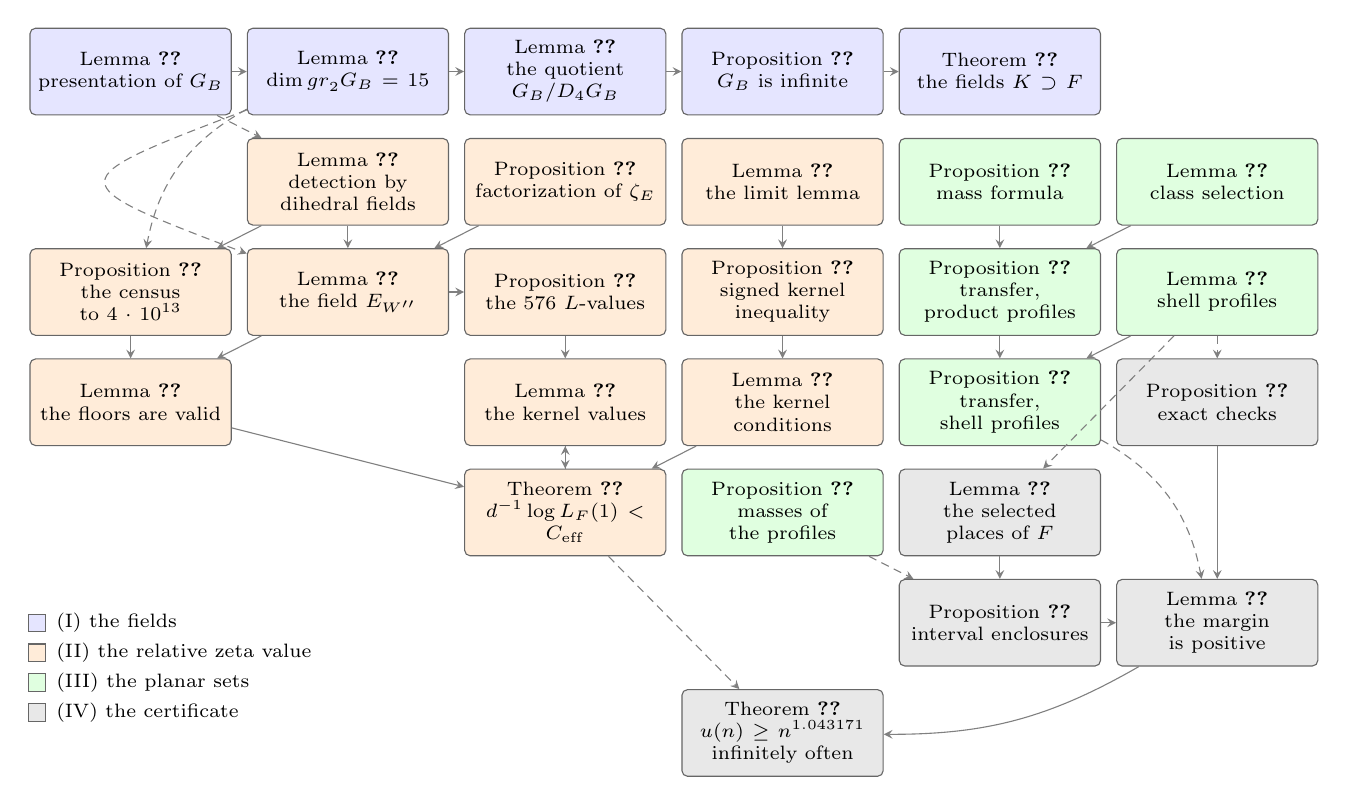
\begin{tikzpicture}[x=1cm,y=1cm,>=stealth,
 box/.style={draw=black!60,rounded corners=2pt,align=center,font=\scriptsize,
  execute at begin node={\hyphenpenalty=10000\exhyphenpenalty=10000},
  inner sep=1.5pt,minimum height=1.10cm,text width=2.45cm}]
\node[box,fill=blue!10] (tw-GB-presentation) at (0.000,0.000) {Lemma~\ref*{tw:GB-presentation}\\ presentation of $G_B$};
\node[box,fill=blue!10] (tw-quadratic-layer) at (2.760,0.000) {Lemma~\ref*{tw:quadratic-layer}\\ $\dim\operatorname{gr}_2G_B=15$};
\node[box,fill=blue!10] (tw-retained-quotient) at (5.520,0.000) {Lemma~\ref*{tw:retained-quotient}\\ the quotient $G_B/D_4G_B$};
\node[box,fill=blue!10] (tw-infinite) at (8.280,0.000) {Proposition~\ref*{tw:infinite}\\ $G_B$ is infinite};
\node[box,fill=blue!10] (tw-field-family) at (11.040,0.000) {Theorem~\ref*{tw:field-family}\\ the fields $K\supset F$};
\node[box,fill=orange!15] (dh-detection) at (2.760,-1.400) {Lemma~\ref*{dh:detection}\\ detection by dihedral fields};
\node[box,fill=orange!15] (gf-factorization) at (5.520,-1.400) {Proposition~\ref*{gf:factorization}\\ factorization of $\zeta_E$};
\node[box,fill=orange!15] (an-limit) at (8.280,-1.400) {Lemma~\ref*{an:limit}\\ the limit lemma};
\node[box,fill=orange!15] (dh-census) at (0.000,-2.800) {Proposition~\ref*{dh:census}\\ the census to $4\cdot10^{13}$};
\node[box,fill=orange!15] (dh-EW) at (2.760,-2.800) {Lemma~\ref*{dh:EW}\\ the field $E_{W''}$};
\node[box,fill=orange!15] (lv-values) at (5.520,-2.800) {Proposition~\ref*{lv:values}\\ the $576$ $L$-values};
\node[box,fill=orange!15] (an-signed) at (8.280,-2.800) {Proposition~\ref*{an:signed}\\ signed kernel inequality};
\node[box,fill=orange!15] (dh-floors-valid) at (0.000,-4.200) {Lemma~\ref*{dh:floors-valid}\\ the floors are valid};
\node[box,fill=orange!15] (ce-values) at (5.520,-4.200) {Lemma~\ref*{ce:values}\\ the kernel values};
\node[box,fill=orange!15] (ce-kernel) at (8.280,-4.200) {Lemma~\ref*{ce:kernel}\\ the kernel conditions};
\node[box,fill=orange!15] (an-ceiling) at (5.520,-5.600) {Theorem~\ref*{an:ceiling}\\ $d^{-1}\log L_F(1)<C_{\rm eff}$};
\node[box,fill=green!12] (geo-mass) at (11.040,-1.400) {Proposition~\ref*{geo:mass}\\ mass formula};
\node[box,fill=green!12] (geo-selection) at (13.800,-1.400) {Lemma~\ref*{geo:selection}\\ class selection};
\node[box,fill=green!12] (geo-transfer) at (11.040,-2.800) {Proposition~\ref*{geo:transfer}\\ transfer, product profiles};
\node[box,fill=green!12] (fw-shell-lemma) at (13.800,-2.800) {Lemma~\ref*{fw:shell-lemma}\\ shell profiles};
\node[box,fill=green!12] (fw-transfer) at (11.040,-4.200) {Proposition~\ref*{fw:transfer}\\ transfer, shell profiles};
\node[box,fill=green!12] (pf-mass) at (8.280,-5.600) {Proposition~\ref*{pf:mass}\\ masses of the profiles};
\node[box,fill=gray!18] (cert-exact) at (13.800,-4.200) {Proposition~\ref*{cert:exact}\\ exact checks};
\node[box,fill=gray!18] (cert-places) at (11.040,-5.600) {Lemma~\ref*{cert:places}\\ the selected places of $F$};
\node[box,fill=gray!18] (cert-enclosures) at (11.040,-7.000) {Proposition~\ref*{cert:enclosures}\\ interval enclosures};
\node[box,fill=gray!18] (cert-lower-margin) at (13.800,-7.000) {Lemma~\ref*{cert:lower-margin}\\ the margin is positive};
\node[box,fill=gray!18] (thm-main) at (8.280,-8.400) {Theorem~\ref*{thm:main}\\ $u(n)\ge n^{1.043171}$ infinitely often};
\draw[->,black!50] (an-ceiling) -- (ce-values);
\draw[->,black!50,densely dashed] (an-ceiling) -- (thm-main);
\draw[->,black!50] (an-limit) -- (an-signed);
\draw[->,black!50] (an-signed) -- (ce-kernel);
\draw[->,black!50] (ce-kernel) -- (an-ceiling);
\draw[->,black!50] (ce-values) -- (an-ceiling);
\draw[->,black!50] (cert-enclosures) -- (cert-lower-margin);
\draw[->,black!50] (cert-exact) -- (cert-lower-margin);
\draw[->,black!50] (cert-lower-margin) to[bend left=15] (thm-main);
\draw[->,black!50] (cert-places) -- (cert-enclosures);
\draw[->,black!50] (dh-EW) -- (dh-floors-valid);
\draw[->,black!50] (dh-EW) -- (lv-values);
\draw[->,black!50] (dh-census) -- (dh-floors-valid);
\draw[->,black!50] (dh-detection) -- (dh-EW);
\draw[->,black!50] (dh-detection) -- (dh-census);
\draw[->,black!50] (dh-floors-valid) -- (an-ceiling);
\draw[->,black!50,densely dashed] (fw-shell-lemma) -- (cert-exact);
\draw[->,black!50,densely dashed] (fw-shell-lemma) -- (cert-places);
\draw[->,black!50] (fw-shell-lemma) -- (fw-transfer);
\draw[->,black!50,densely dashed] (fw-transfer) to[bend left=25] (cert-lower-margin);
\draw[->,black!50] (geo-mass) -- (geo-transfer);
\draw[->,black!50] (geo-selection) -- (geo-transfer);
\draw[->,black!50] (geo-transfer) -- (fw-transfer);
\draw[->,black!50] (gf-factorization) -- (dh-EW);
\draw[->,black!50] (lv-values) -- (ce-values);
\draw[->,black!50,densely dashed] (pf-mass) -- (cert-enclosures);
\draw[->,black!50,densely dashed] (tw-GB-presentation) -- (dh-detection);
\draw[->,black!50] (tw-GB-presentation) -- (tw-quadratic-layer);
\draw[->,black!50] (tw-infinite) -- (tw-field-family);
\draw[->,black!50,densely dashed] (tw-quadratic-layer) .. controls (-0.920,-1.400) .. (dh-EW);
\draw[->,black!50,densely dashed] (tw-quadratic-layer) to[bend right=25] (dh-census);
\draw[->,black!50] (tw-quadratic-layer) -- (tw-retained-quotient);
\draw[->,black!50] (tw-retained-quotient) -- (tw-infinite);
\node[draw=black!60,fill=blue!10,minimum size=0.22cm,inner sep=0pt] at (-1.190,-7.000) {};
\node[anchor=west,font=\scriptsize,inner sep=0pt] at (-0.950,-7.000) {(I) the fields};
\node[draw=black!60,fill=orange!15,minimum size=0.22cm,inner sep=0pt] at (-1.190,-7.380) {};
\node[anchor=west,font=\scriptsize,inner sep=0pt] at (-0.950,-7.380) {(II) the relative zeta value};
\node[draw=black!60,fill=green!12,minimum size=0.22cm,inner sep=0pt] at (-1.190,-7.760) {};
\node[anchor=west,font=\scriptsize,inner sep=0pt] at (-0.950,-7.760) {(III) the planar sets};
\node[draw=black!60,fill=gray!18,minimum size=0.22cm,inner sep=0pt] at (-1.190,-8.140) {};
\node[anchor=west,font=\scriptsize,inner sep=0pt] at (-0.950,-8.140) {(IV) the certificate};
\end{tikzpicture}
\caption{The structure of the proof (Subsection~\ref{intro:structure}). Each box is a numbered statement, coloured by the part of the proof it belongs to. An arrow goes from a statement to each statement whose proof uses it, directly or through statements not shown, except that arrows implied by a chain of drawn arrows are left out; dashed arrows join different parts. The arrows from Theorem~\ref{tw:field-family}, which supplies the fields to which Parts (II)--(IV) apply, are also left out. Appendix~\ref{dep:section} lists the citations between all numbered statements; the notation is collected in Subsection~\ref{intro:notation}.}
\label{fig:structure}
\end{figure}
